\chapter{Algorithms as Puzzle Helper}
\label{chap:puzzleHelper}
%Short Intro what I do here

The following chapter explains the first steps towards a puzzle solver algorithm. In the beginning, the characteristics of the dataset and the performed preprocessing steps are explained. Afterward, the necessary theory behind a puzzle helper is explained. Finally, the results of various experiments and their evaluation are presented. The main objective is to show that the algorithm can provide a subset of potential matches for a given papyrus fragment.  

\section{Methods}

\subsection{Data}


Beispielbilder  - Wie sehen die Daten aus? 

\begin{figure}[t]
	\label{fig:sample_grid}
	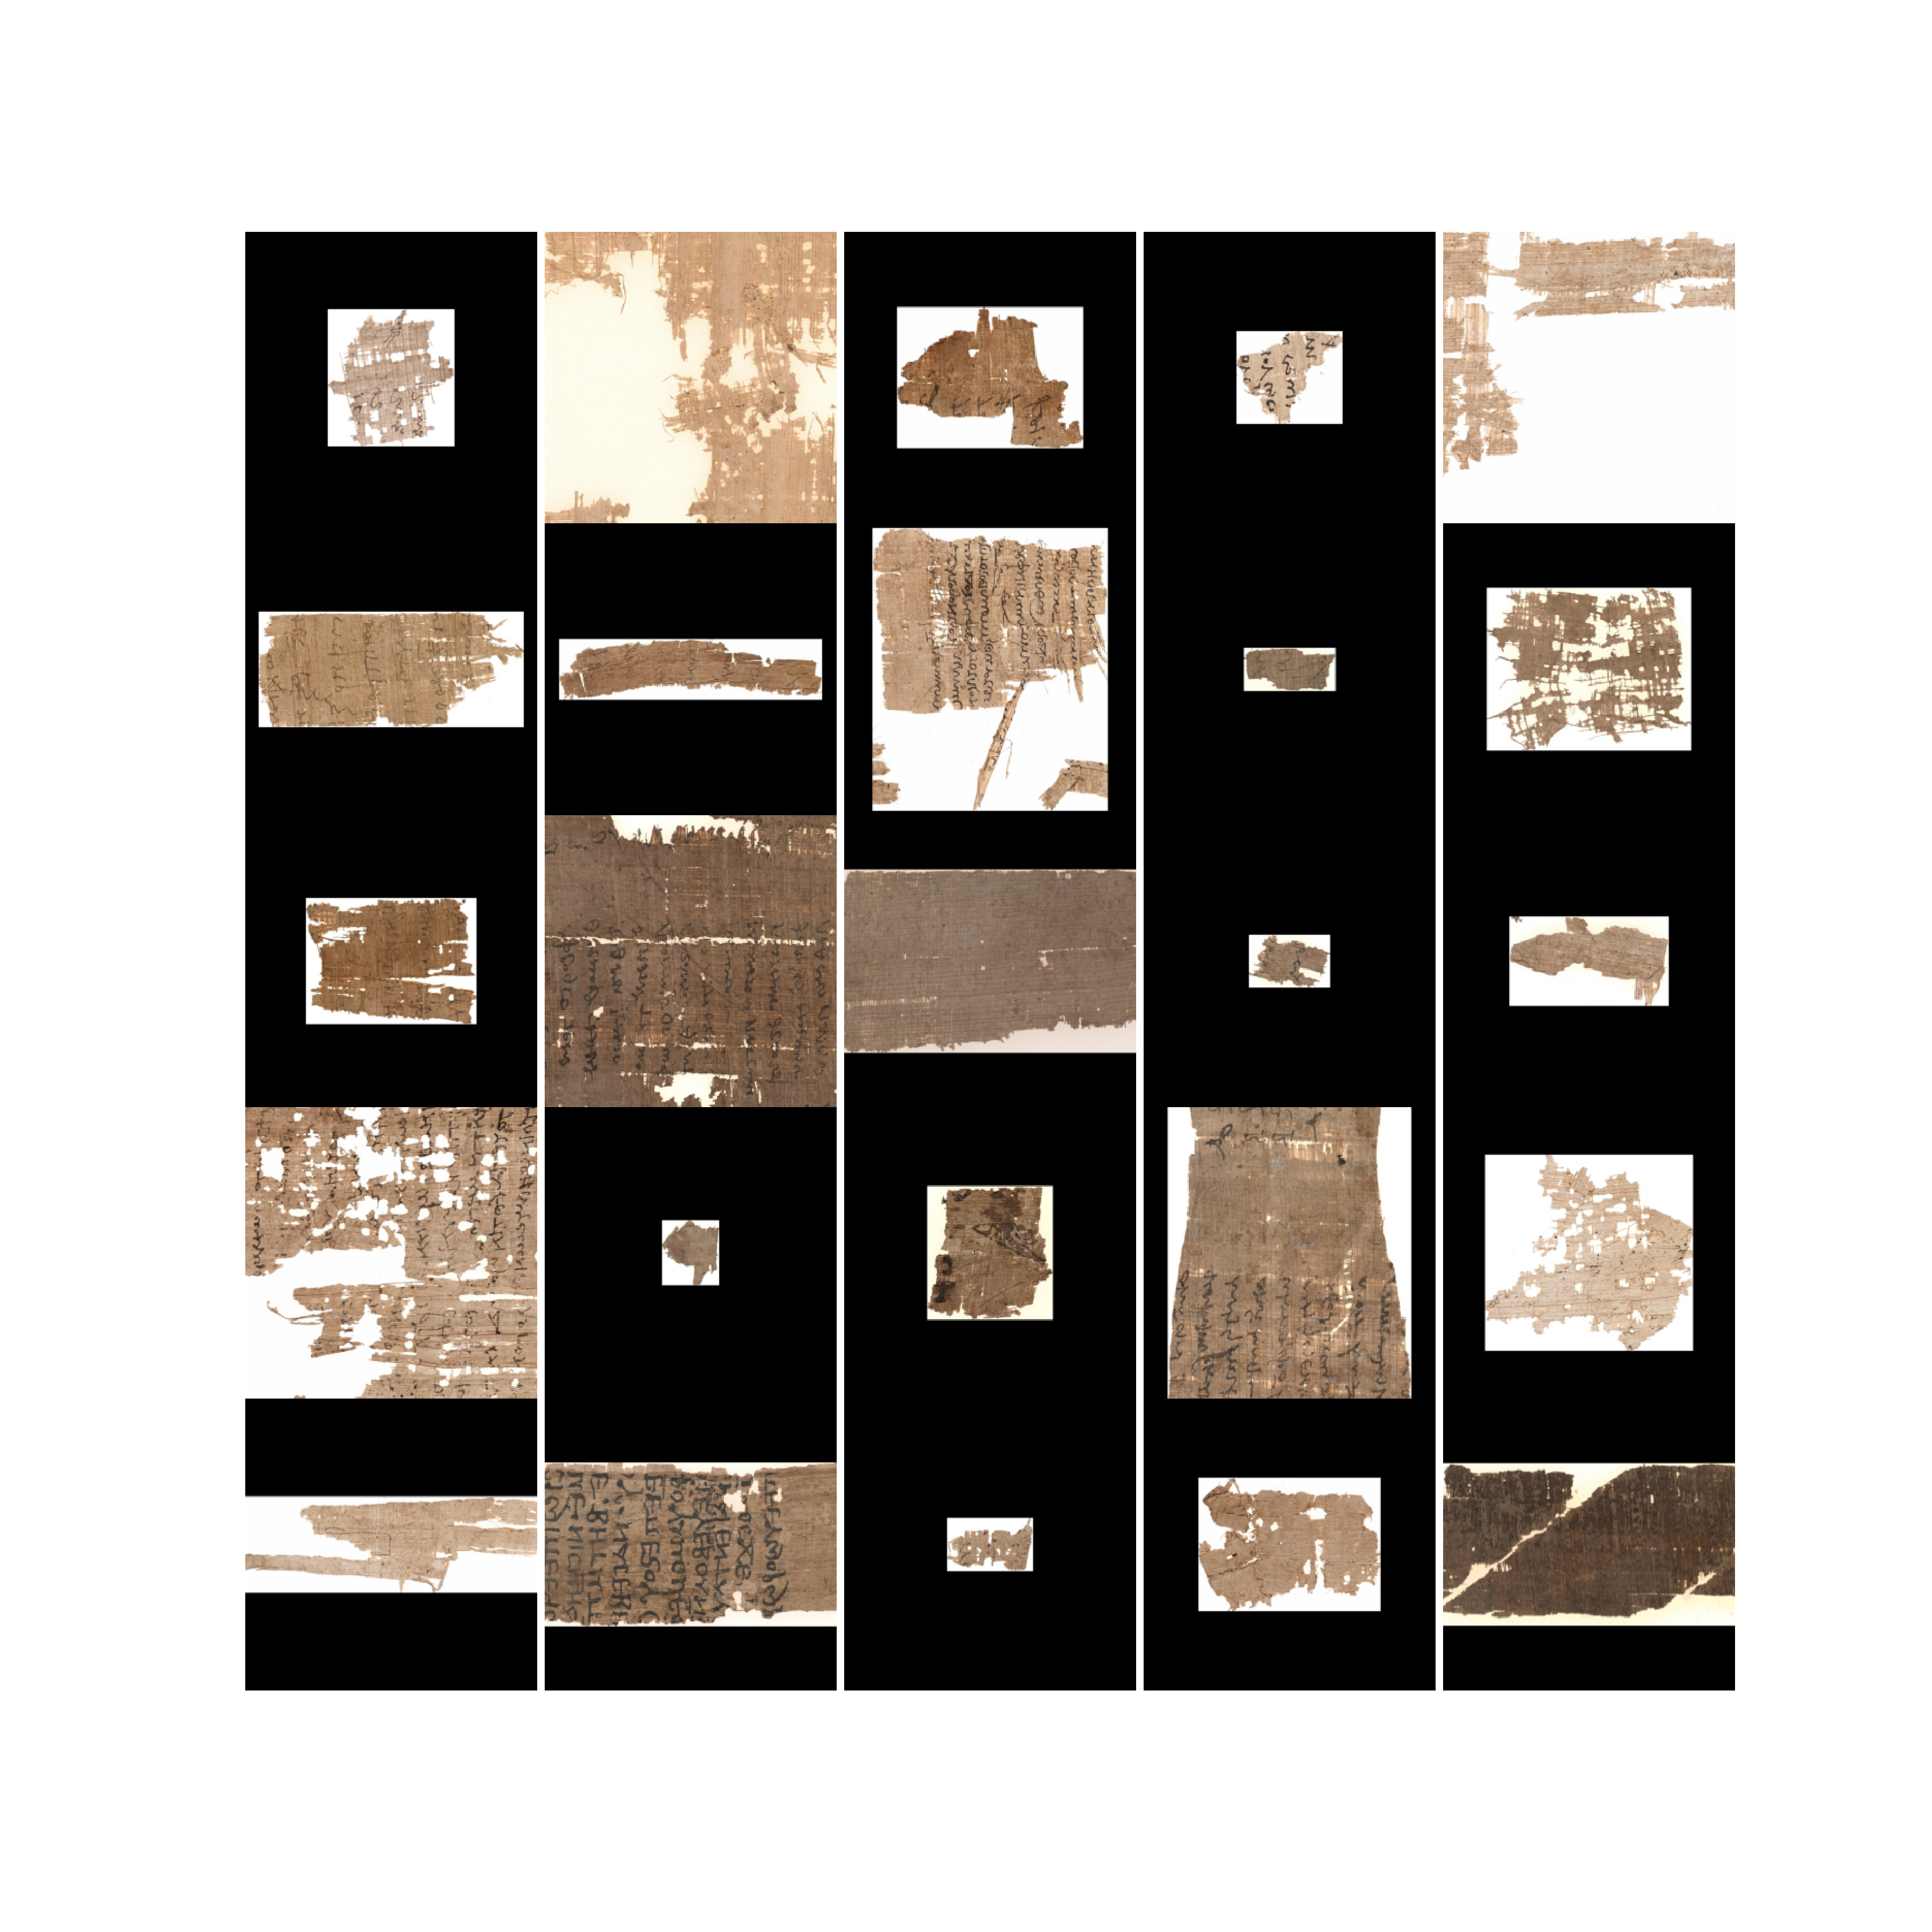
\includegraphics[width=\textwidth]{figures/sample_grid.pdf}
	\caption{Each papyri was turned into grayscale, blured ...}
\end{figure}


Histogram der gedownloadeten Bilder. \ref{fig:hist_orginal} \ref{fig:hist_train} \ref{fig:hist_val} \ref{fig:hist_test}

\begin{figure}[t]
	\label{fig:hist_orginal}
	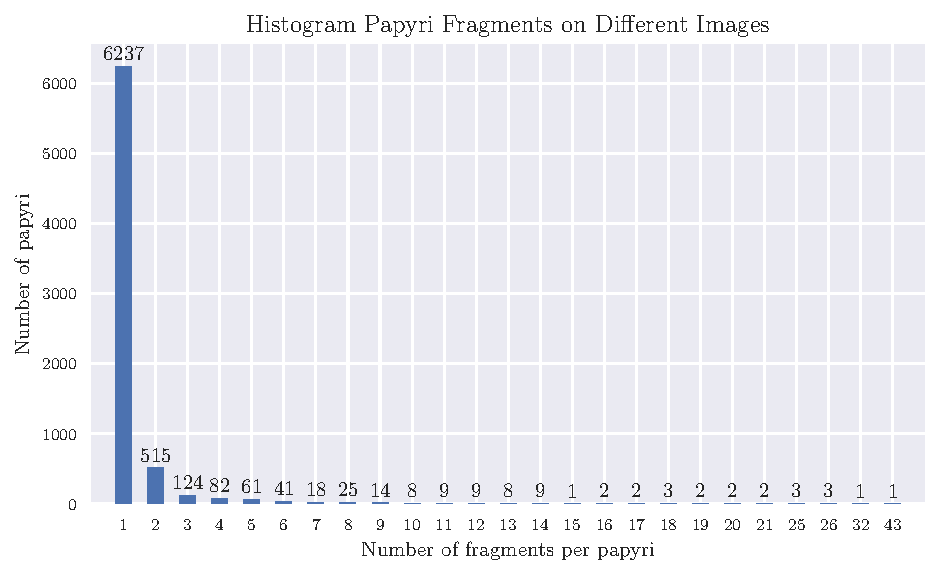
\includegraphics[width=\textwidth]{figures/HistogramFragOriginal.pdf}
	\caption{Each papyri was turned into grayscale, blured ...}
\end{figure}

\begin{figure}[t]
	\label{fig:hist_train}
	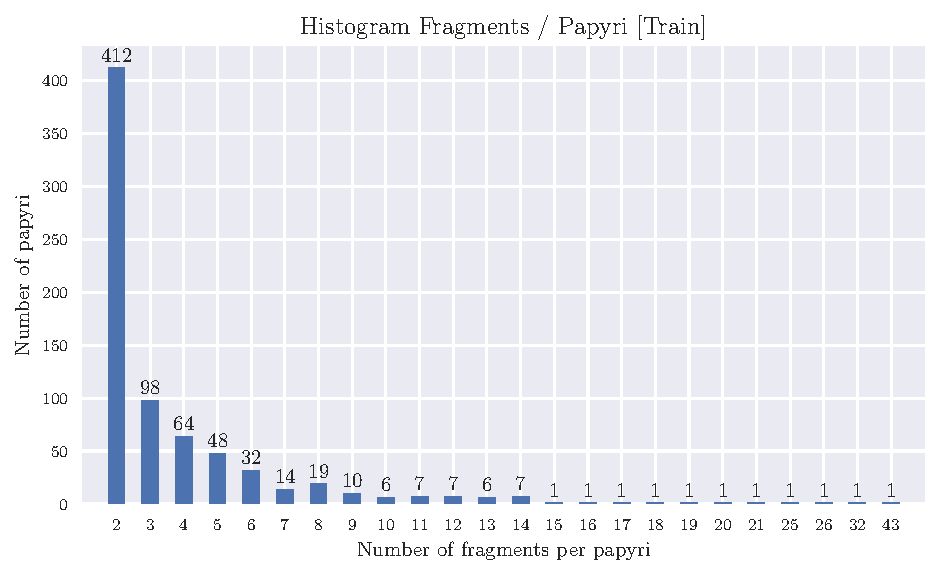
\includegraphics[width=\textwidth]{figures/HistogramFragAfterTrain.pdf}
	\caption{Train Histrogram}
\end{figure}

\begin{figure}[t]
	\label{fig:hist_test}
	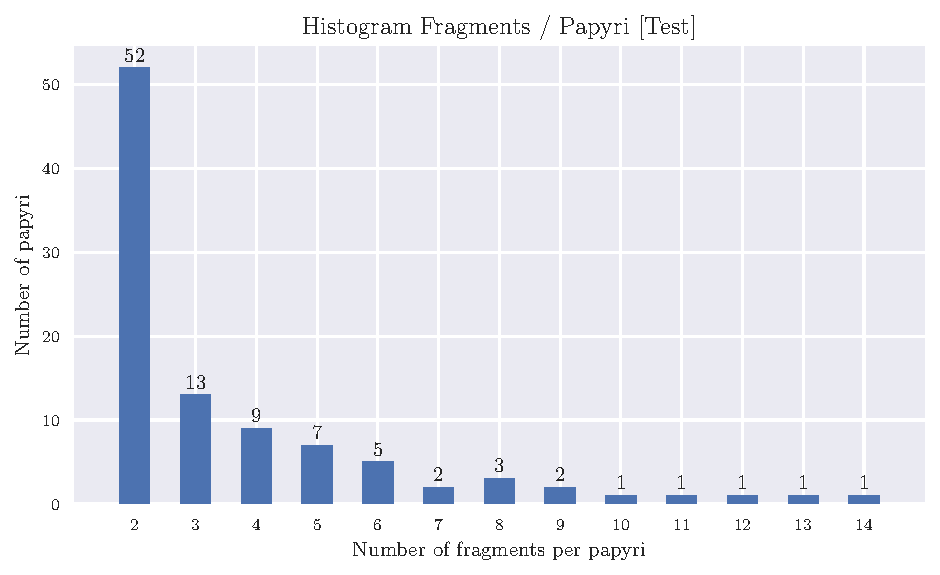
\includegraphics[width=\textwidth]{figures/HistogramFragTest.pdf}
	\caption{Test Histogram}
\end{figure}

\begin{figure}[t]
	\label{fig:hist_val}
	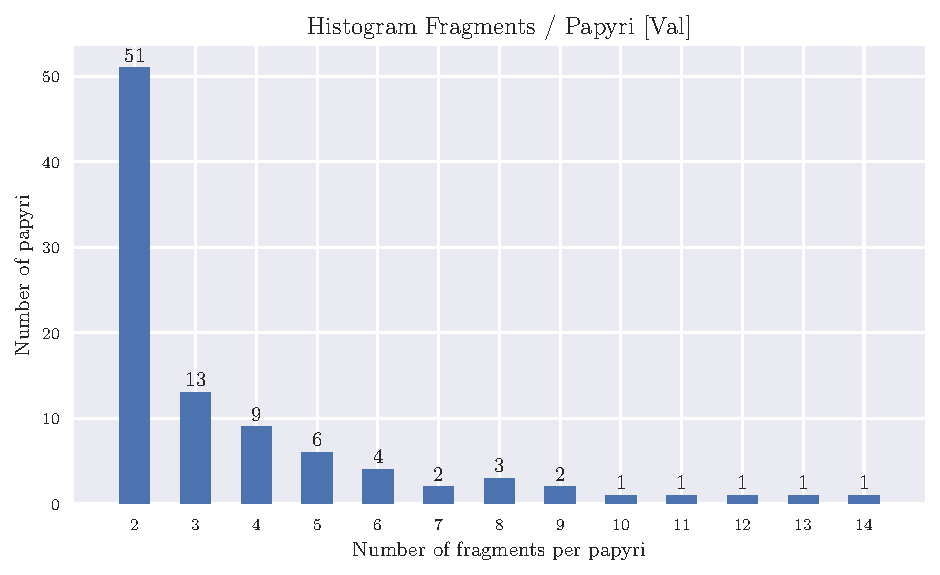
\includegraphics[width=\textwidth]{figures/HistogramFragAfterVal.pdf}
	\caption{Valdidation Histrogram}
\end{figure}

Boxplots für die Grosse. 


Pipelinediagramm \ref{fig:papyri_preprocessing}. Was haben wir mit den Daten gemacht?

\begin{figure}[t]
	\label{fig:papyri_preprocessing}
	\includegraphics[width=\textwidth]{figures/papyri_preprocessing.pdf}
	\caption{Each papyri was turned into grayscale, blured ...}
\end{figure}


Bild metrisches lernen erklären - wie funktioniert unser Algorithmus?


Schaubild Metric Welche Metriken werden verwendet?

Was bedeutet die Zufallsmetrik. 



\section{Results}
% What happend?
Tabelle mit Hyperparametern und Ergebnissen - Welche Experimente wurden durchgeführt? 
Graph mit mAP 

U-MAP
Accuracy Plot?

\section{Evaluation}
Was lief gut?
Was lief schlecht?